\linespread{1.6}
\documentclass[pageno]{jpaper}

% \newcommand{\IWreport}{2015}

\usepackage[normalem]{ulem}
\usepackage{amsmath, adjustbox, geometry, booktabs, tabularx}
\DeclareMathAlphabet{\mathcal}{OMS}{cmsy}{m}{n}
\newcommand{\norm}[1]{\left\lVert#1\right\rVert}
\newcommand{\textbi}[1]{\textbf{\textit{#1}}}

\begin{document}

\title{
Solving SAT Reading Comprehension Questions with Memory Networks}

\author{Saahil Madge\\Adviser: Professor Christiane Fellbaum}

\date{}
\maketitle

\thispagestyle{empty}
\doublespacing
% \begin{abstract}
% This document is intended to serve as a sample you can use for independent work reports.  We provide some guidelines on content and formatting.  They are not required, but they might be helpful.
% \end{abstract}

\section{Background and Motivation}
\label{Background and Motivation}

Machine question-answering (QA) has been a popular subject in recent research.
It is a very interesting field from an academic perspective, requiring
knowledge and techniques across the areas of artificial intelligence, machine
learning, natural language processing, linguistics, and mathematics.

QA has applications to many aspects of daily life. A famous use of
question-answering techniques is in Apple's Siri program. Siri combines speech
recognition software with question-answering techniques to create a virtual
iPhone assistant. Another example is IBM's Watson, which answered questions in
many subjects and performed quite well as a contestant on the game show
\textit{Jeopardy!} A less spectacular but more commonly-used example can be seen
by typing in a simple question such as \textit{How many calories are in an
apple?} on Google. The search results provide a detailed nutritional breakdown
of an apple.

The general term QA covers a broad array of subfields. Information retrieval,
factual question-answering, reading comprehension, and inference are all part
of the greater question-answering area. QA is a rapidly evolving field, but as
the examples above indicate, recent research has focused extensively on
answering spoken questions, and factual questions.

However, the subfield of machine comprehension has not been studied nearly as
well, though it has become quite popular in the past few years. Machine
comprehension involves training programs and systems to read text and answer
questions based on the newly acquired information. In most other QA tasks, the
system has a large database of facts (knowledge base) and must interpret the
question and provide the relevant factual answer. Machine comprehension tasks,
on the other hand, require the system to parse both the informational text as
well as the question, and then provide the correct answer. As there is
possibility for error within the knowledge base, machine comprehension tasks
are some of the most difficult QA tasks.

Machine comprehension has a wide range of applications. Reading comprehension
tests are a natural choice, but fields like document retrieval also use machine
comprehension techniques. Financial firms that use news analysis to make
trading decisions heavily rely on these techniques as well. Many long-term
goals of AI such as dialogue and humanoid robots cannot be achieved without
significant advance in this area \cite{Weston2015}. Another incentive to
study machine comprehension is that new research here can be applied to drive
research in many other areas of artificial intelligence and natural language
processing.

As a consequence of machine comprehension tasks being so difficult, most
research with reading comprehension tests has focused on elementary school
level tests. The most common dataset is MCTest\cite{Richardson2013}, which we
discuss in more detail in \ref{Related Work}. This dataset is a set of passages
and reading comprehension questions created by crowdsourcing. The stories are
``carefully limited to those a young child would
understand''\cite{Richardson2013}. Another common dataset is Facebook's bAbi
dataset\cite{Weston2015}, which has a collection of short toy problems that can
be used to train machine comprehension systems. These problems could certainly
be solved by a human elementary school student. Berant et al.\cite{Berant2014}
train a system to answer questions based on a paragraph describing biological
processes, which is certainly an advanced topic, but the system is specialized
for biological tasks and not applicable as is to general reading comprehension.

In this paper we focus on SAT reading questions. The major reason is that they
are far more complex than MCTest questions and other commonly-used machine
comprehension datasets. The sentence structures, vocabulary, and topics covered
in SAT passages are all far more varied than in the other benchmarks. The
questions are much harder as well, and simply understanding the question and the
individual choices is difficult by itself. SAT questions often test underlying
themes and broad ideas rather than particular factual details (``Why'' or
``How'' questions). In contrast, MCTest questions are often of a ``Who'',
``When'', or ``What'' form, which have traditionally been easier for programs to
answer.

Another aspect that makes SAT questions so difficult is that they require
inference to answer, as opposed to just matching words or syntax. MCTest and
similar questions can mostly be answered through word-matching (discussed in
\ref{Bag-of-words}) or via syntactic matching. Word-matching means the system
will try to find which sentences in the passage have the most words in common
with the query, and use that to choose an answer. Syntactic matching is the same
principle, but aims to match syntactic structure. SAT questions, however, almost
never repeat the answer words in the question itself, and the query structure is
not correlated with passage structure. To solve these questions, our system has
to really understand the high-level concepts and information that is implied but
not directly on the surface. This is a significantly harder problem than has
been tackled before, but it is necessary to solve to continue moving forwad in
the field of machine comprehension. Essentially, by trying to answer SAT
questions we can try to solve problems that will be present in real-world
applications but have not yet been tackled by existing research.

Due to the difficulty of interpreting the text as-is, we represent the text
using relational logic instead. Essentially we dynamically create a
\textit{Knowledge Graph} (covered in more detail in \ref{Representation
Techniques}) as we parse through the text and try to frame each question as a
query on this knowledge graph. The knowledge graph representation is typically
used for factual data that has already been collected in entity-relation triple
form. As far as we know, no previous research in this space has tried to
dynamically create a knowledge graph on which we can answer questions.

Traditionally most research on relational learning has used either neural
networks or tensor decomposition to answer queries on the graph. In this work we
present an improved version of both methods. For tensor factorization we enhance
a method known as RESCAL\cite{Bader2007}\cite{Nickel2011} with a technique known
as \textit{Semantically Smooth Embedding}\cite{Guo2015}. RESCAL trains a
factorization of the knowledge graph using Alternating Least Squares, and this
factorization can then be used to answer queries.

The neural network approaches such as TransE\cite{Bordes2013} and
TransH\cite{Wang2014} use neural networks to train an embedding method for the
relations on the knowledge graph, and use the trained model to answer queries.
However, none of these previous approaches are designed for question-answering.
We enhance the Memory Networks architecture proposed by Weston et
al.\cite{Weston2015a} and improved by Sukhbaatar et al.\cite{Sukhbaatar2015} to
take knowledge graph triples and queries as input, and provide a scoring of the
answer choices as output. We discuss memory networks and alternatives in much
greater depth in \ref{Related Work} and \ref{Model}.

Our goal with this research is to present a way to combine ideas that were
previously used in isolation for QA or other learning tasks into a system which
can parse and interpret a complex text, and answer difficult high-level
questions about the text. The text, questions, and techniques we use are more
ambitious than those studied in previous research. Our results should be
interpreted as merely proof-of-concept. We hope that this paper will encourage
others to tackle problems of equal or greater ambition, and drive progress in
the development of safe artificial intelligence.

\section{Technical Review}
\label{Technical Review}

In this section we review some of the techniques that are used in previous
research and in this paper.

\subsection{Representation Techniques}
\label{Representation Techniques}

We begin by reviewing various methods for embedding text and performing queries
on the embedded representations. \\

\subsubsection{Bag-of-words}
\label{Bag-of-words}

Bag-of-words is a type of analysis in which we treat each sentence as simply a
collection of words, without paying attention to their order or the dependencies
between individual words. If we have some vocabulary of size $V$, we can encode
each sentence as a vector of size $V$ where each vector element corresponds to
some word in the vocabulary. If the word appears in the sentence we store how
many times it appears, and if it does not appear we store it as a 0. This is
known as \textit{one-hot} vector encoding. Most designs encode each input
sentence and the query as one-hot vectors. These vectors are not used as-is, but
are first embedded into some dimension $d$. The learning algorithm is run on the
embedded vectors, and we can output a response in a specified format. Two common
methods are to return a probability vector of size $V$ where each element
represents how likely that word is to be the output, or to pick the most likely
word from that distribution and return only that word. \\

\subsubsection{Dependency Parsing}
\label{Dependency Parsing}

Dependency parsing is an important technique used to understand the structural
information in a sentence. Essentially, dependency parsing creates a graph of
the words in the sentence and describes how each word relates to other words. A
sample graph is shown in Figure~\ref{fig: dependency parsing}. Each dependency
in the graph has a \textit{governor} and \textit{dependent}. The collection of
dependencies contains all the structural relationships in the sentence. Each
dependency is labelled to show the exact relationship between governor and
dependent. For example, in the graph in Figure~\ref{fig: dependency parsing} the
label \textit{nsubj} highlights the nominal subject of a particular clause in
the sentence\cite{De2014}. The specific parser we use is the Stanford
High-Performance Dependency Parser by Chen and Manning\cite{Chen2014}.

Once the dependency graph is created, we can analyze it to extract the relevant
information in the sentence. The exact details are discussed more in Section
\ref{Converting to Knowledge Graph Representation}. The basic approach is to
find the main subject of the sentence and either the direct object it acts on
or some description of it. Then it can be turned into an entity-relation triple
on the knowledge graph.

\subsubsection{word2vec}
\label{word2vec}

The \textit{word2vec} embedding technique introduced by Mikolov et al.
\cite{Mikolov2013} is perhaps the most common embedding technique used in NLP
research. It is actually an umbrella term for various methods, such as
\textit{skip-gram} or even bag-of-words embedding. The word2vec techinque
produces a vector representation of words, often with several hundred elements.
These representations can then be manipulated as vectors in the
higher-dimensional space, allowing for interesting operations on words. For
example, \textbf{vector(``king'')} - \textbf{vector(``man'')} +
\textbf{vector(``woman'')} produces a vector that is very close to
\textbf{vector(``queen'')}. The reason word2vec is able to embed so successfully
is generally thought to be the fact that the process of embedding gives
similar words a similar embedding (which is measured by cosine similarity). \\

\subsubsection{Knowledge Graph}
\label{Knowledge Graph}

A knowledge graph generally refers to a set of \textit{entity-relation triples}.
These triples take the form $\langle e_1, r, e_2 \rangle$. where $e_1$ and $e_2$
are entities and $r$ describes the relation between these two entities. Entities
and relations can be repeated across triples. The total set of triples denotes
all the knowledge in our ``Knowledge Base''.

\begin{figure}
    \centering
    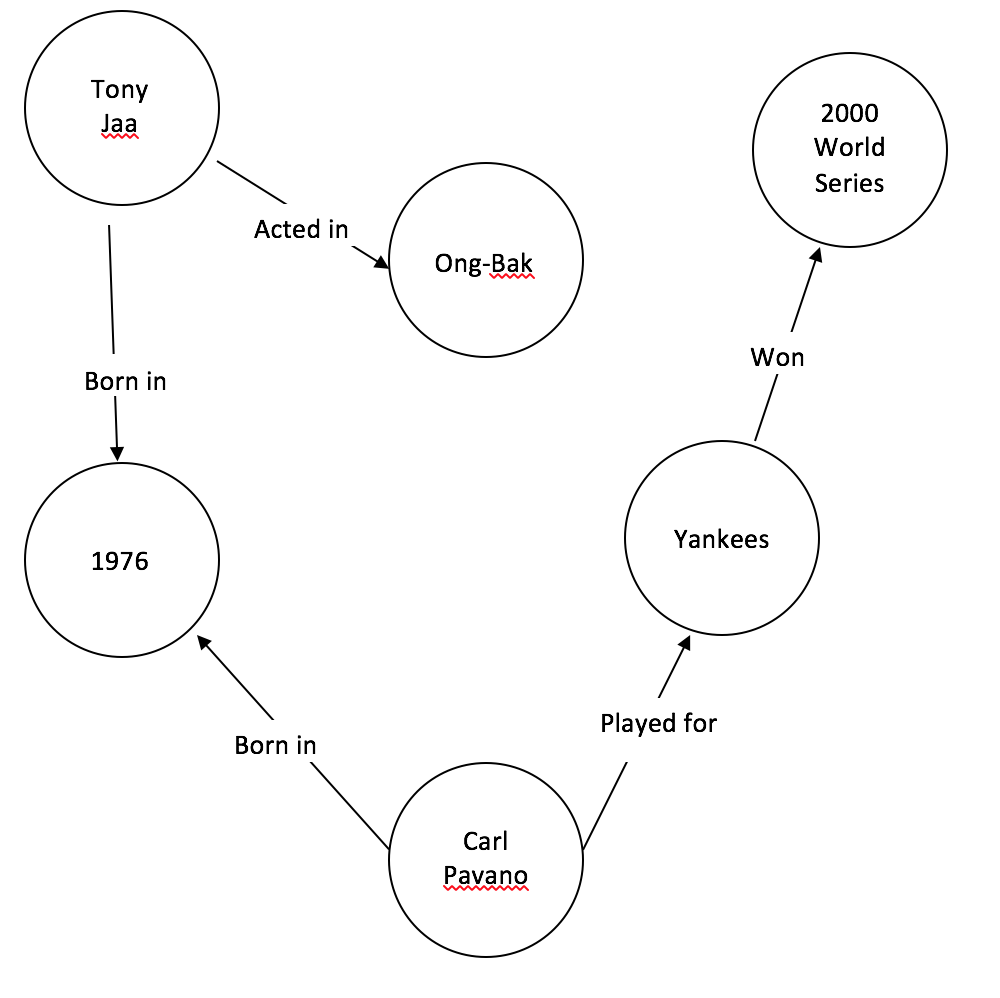
\includegraphics[width=0.7\textwidth,keepaspectratio]{figures/Example_KG.png}
    \caption{A small example knowledge graph}
    \label{Figure: KG}
\end{figure}

We can represent these triples as a directed graph, with each entity as a vertex
and the relations as edge types between them. Figure \ref{Figure: KG} shows an
example of a very small knowledge graph. Note that there is only one node per
entity. This allows the graph to store multiple pieces of information regarding
the same entity together, to allow for easy processing by the program while also
making it simple for humans to understand. The mathematical details of our
knowledge graph model can be found in \ref{Model}.

Once a knowledge graph is built, we can pose queries about the graph. For
example, we can provide two entities $e_1$, $e_2$ and ask which relation $r$
links the two on the graph. We can also provide an entity $e$ and the relation
$r$, and ask for which other entity $e'$ do the triples $\langle e,r,e' \rangle$
or $\langle e',r,e \rangle$ exist on the graph. Put another way, the queries are
either \textit{link prediction} queries or \textit{entity prediction} queries.

\subsection{Neural Networks}
\label{Neural Networks}

As discussed in \ref{Background and Motivation}, recent research in machine
comprehension has extensively used neural nets (NNs) and their variants. Here we
provide a quick review of neural network design. These topics can be covered in
far more depth in \cite{Bishop1995} and \cite{Nielsen2015}.

The most basic model is known as a \textit{feed-forward} neural net. These have
several layers composed of units (nodes). There is an initial input layer, a
final output layer, and \textit{hidden layers} in the middle. A unit in layer
$l$ takes as input the output of nodes in the previous layer (or the actual
input if this is the input layer). It multiplies these by some weight matrix
$W^l$, transforms it using an activation function $g$, and sends its output to the
next layer (or as the final output if this is the output layer). Common
activation functions are the $tanh$ and $sigmoid$ functions. The sigmoid
function is defined as $\sigma (x) = \frac{1}{1+e^{-x}}$. For now we will assume
that our activation function is sigmoid.

Mathematically, we define the input to the current layer as $x^{l-1}$,
where $x^{l-1}_{ij}$ means that it is the input from unit $j$ in the previous
layer to unit $i$ in the current layer. $W^l_{ij}$ is the weight on this
connection, defined as 0 if node $i$ does not depend on node $j$. The output of
node $j$ is $\sigma ( W^l x^{l-1}_j)$. Typically the quantity $Wx^{l-1}_j$ is
known as $z_j$. We can also define bias vectors $b$ such that $z_j =
W^lx^{l-1}_j + b^l_j$. To summarize, we can write the output of some layer $l$
in vector notation as
$$o^l = \sigma(W^lx^{l-1} + b^l)$$

We can propagate this forward starting at the input layer, through the hidden
layers, and finally at our output layer. We can then train our network using the
backpropagation algorithm. We have some cost function $C$ that is a measure of
the error of our output. We find the error at the output layer, and then change
the weights at each previous layer, working backwards to the input layer. The
key to backpropagation relies on updating the weights based on their partial
derivatives with relation to $C$. In-depth derivations are provided in
\cite{Bishop1995} and \cite{Nielsen2015}.\\

\subsubsection{Recurrent Neural Networks}
\label{Recurrent Neural Networks}

Feed-forward networks are good tools, but do not have any form of state
(memory). Here we review recurrent neural networks (RNNs) which have a hidden
state $h_t$.

At step $t$ in a recurrent neural network, we have input $x_t$ and a hidden
state $h_{t-1}$. We also have weight matrices $U$ and $W$. We can define the
current state $h_t = \sigma(Ux_t + Wh_{t-1})$. We have another weight matrix $V$
for the output. The output $y_t = softmax(h_t)$, where $softmax(z_i) =
\frac{e_{z_i}}{\sum_j e^{z_j}}$. The softmax function output is a probability
distribution over the vector.

Using the softmax function has several advantages. Because it is a smooth
function, we can take its derivative, making it easier to calculate the
backpropagation equations. Additionally, most RNNs and variants use a loss
function known as cross-entropy loss. If the model output is $\hat{y}$ and the
real (target) is $y$, then cross-entropy loss is defined as $\sum_i y_i
\log(\hat{y_{i}})$. When we pair a softmax output with cross-entropy loss, the
error at the output node $i$ is simply $\hat{y_i} - y_i$. This is very
convenient because it can be calculated rapidly, so it allows for fast training
of the RNN. Training is normally a bottleneck, and by combining a robust output
function and robust loss function we get a very elegant output error. As this is
a very important result, we have included it in \ref{Derivation of Output Layer
Error}.

\section{Related Work}
\label{Related Work}

The first major research in machine comprehension was conducted by Hirschman,
et al.\cite{Hirschman1999}. Their system ``Deep Read'' takes a story and a
series of questions as input, and proposes answers by using bag-of-words
techniques with other methods such as stemming and pronoun resolution layered
on top. On a collection of remedial reading questions for grades 3-6, Deep Read
answered about 40\% of the questions correctly.

Most recent research has used the MCTest\cite{Richardson2013}, released by
Richardson, et al. at Microsoft research. There are a total of 500 passages,
each with 400 questions, created at the reading level of a young child. The
stories are fictitious, which means the answers can only be found in the story
itself. Richardson et al. also provide two baseline implementations to serve as
a benchmark. The first is a simple bag-of-words model with a sliding window. It
scores about 51\% accuracy on the MC500 questions. The second implementation
adds a distance-based scoring metric and reaches 56\% accuracy. Both
implementations score significantly higher on questions where the answer is
contained in just one sentence than on questions where the answer requires
information across multiple sentences.

Narasimhan and Barzilay\cite{Narasimhan2015} also work on the MCTest tasks.
Their main insight is to create a task-specific discourse parser to capture
specific discourse relations in the MCTest passages, while the prevailing
method had been to use generalized off-the-shelf discourse parsers. They create
three models of increasing complexity. The first assumes each question can be
answered using just one sentence, and estimates a joint probability
distribution across the question, query, and answer. The second model adds in
the joint distribution across a second sentence as well, to handle the case in
which the answer needs two sentences to answer. The third model incorporates
discourse relations between the two sentences to better understand the
relationship between information in each sentence. The relations are defined as
``Causal'', ``Temporal'', ``Explanation'', and ``Other''. Most systems have
performed the worst on these types of questions. By focusing specifically on
modeling these explanatory relations, the third model easily outscores the
other two, and the two MCTest baseline implementations, achieving almost 64\%
accuracy.

Berant et al.\cite{Berant2014} also focus on analyzing inter-sentence
relations, with application specifically to passages and questions about
biological processes. These passages generally describe a chemical reaction or
other process in which there are various starting entities which interact with
each other and form a new output. Understanding how the inputs interact and
tracing the flow of the process is crucial to answering the question. To solve
this, Berant et al. define events (or non-events) as ``triggers'', and try to
find relationships between events. The events can be thought of as nodes on a
graph, with an edge defining some relation between the two. There are eight
possible relations, including ``cause'', ``enable'', and ``prevent''. They
first create events and then predict relations between the events. The queries
are also formulated as a graph. They are categorized as dependency questions,
temporal questions, or true-false questions. This model scores almost 67\% on
the dataset, over 6\% better than the next-best model.

Most recent machine comprehension research has focused on using neural nets as
the core system. Neural nets are a very generalizable technique and in the past
decade have become very popular. In fact, advances in neural net techniques have
greatly contributed to the recent surge in machine comprehension research.

Weston et al.\cite{Weston2015a} introduced memory networks. These are a type of
neural network which simulate a long-term memory. We discussed in \ref{Recurrent
Neural Networks} how RNNs have a ``vanishing gradient'' problem, and are not
able to take advantage of states from more than a few steps prior. Memory
networks have a memory module which stores old memories and then updates them
given new inputs. When given a query, the memory network finds relevant
memories, then finds memories that are relevant given those memories, and so on.
Finally, it provides an answer to the query. Sukhbaatar et
al.\cite{Sukhbaatar2015} improved this model by creating a model that can be
trained end to end, while in the original design each module needed to be
trained independently. This is the model that is the basis for our design, so we
discuss it in more detail in \ref{Model}. Kumar et al.\cite{Kumar2015} create
``Dynamic Memory Networks''. Their design uses two memory modules. The semantic
memory module stores general knowledge, while the episodic memory module
iteratively finds memories relevant to the query.

Knowledge Graphs are also a popular research area. There are two main approaches
that are used for solving knowledge graph embedding and query problems. The
first is the neural network embedding style, popularized by Bordes et
al.\cite{Bordes2013} and improved by Wang et al.\cite{Wang2014}. Bordes' TransE
and Wang's TransH both train a neural network to recognize triple embeddings in
some higher dimension. The triples are embedded in such a way that triples that
are ``similar'' according to some metric are embedded near each other. Queries
can be answered more easily using the embedded vectors.

The second approach focuses on representing the knowledge graph as a tensor.
Nickel et al.\cite{Nickel2011} proposed RESCAL, a model which converts the
knowledge graph into a tensor of adjacency matrices and trains a latent rank-$r$
factorization of the tensor using a technique called ASALSAN\cite{Bader2007}.
Queries about the knowledge graph can be easily converted into searching over a
relevant subset of elements in the factorization. Chang et al.\cite{Chang2014}
created TRESCAL, which is an optimized version of RESCAL.

\section{Model}
\label{Model}

This research presents three fundamental insights. \\

\begin{enumerate}

    \item We treat the input text as a knowledge base and dynamically convert it
    into a knowledge graph. We can then interpret the questions as queries on
    the graph, requiring us to find an entity or relation that represents the
    answer to the question. \\

    \item We use tensor decomposition to embed the knowledge graph and
    questions. Specifically, we use an enhanced version of
    RESCAL\cite{Nickel2011}. RESCAL by itself is a fine model, but we make it
    more accurate by adding ``Semantically Smooth Embedding''(SSE), as proposed
    by Guo et al.\cite{Guo2015}. In their original paper they propose adding
    this type of embedding to tensor decomposition as future work, so to our
    knowledge we are the first to perform tensor decomposition with SSE. \\

    \item We embed the knowledge graph and questions into input vectors, and
    pass them into a Memory Network. Given a set of embedded inputs and queries,
    this type of neural network takes advantage of ``memory'' to find new facts
    that are relevant given the current set of relevant facts, but may not be
    relevant solely based on the query. \\

\end{enumerate}

These techniques were first introduced in previous research. However, all of
them were applied to separate domains. Neural nets have been used for machine
comprehension on MCTest, bAbi, and questions of similar difficulty. Their
embedding model is quite simple, however (often just bag-of-words). Knowledge
graphs and tensor decomposition have traditionally been used only for relational
learning when a knowledge graph or set of triples already exists. As our problem
is more complex than that tackled by these original models, and we must combine
these original models, we have to significantly modify their conceptual and
mathematical basis.

\subsection{Knowledge Graph Representation}
\label{Knowledge Graph Representation}

The first part of our design is to dynamically convert the input passage into a
knowledge graph and the questions as queries on that graph. \\

\subsubsection{Advantages of Knowledge Graph Representation}
\label{Advantages of Knowledge Graph Representation}

There are several advantages to using a knowledge graph representation. The main
benefit is that it actually preserves the meaning of the text. Whereas
bag-of-words loses the ordering of words and word2vec keeps the latent
properties but no others, a knowledge graph representation almost completely
stores the intended meaning of the original text. Most sentences in English can
be broken down into Subject-Verb-Object triples, which require little if any
processing to convert into the $\langle \textit{entity}_1, \, \textit{relation}, \,
\textit{entity}_2 \rangle$ format. The knowledge graph itself is simply a list of
these triples. If we can parse the input text and extract the
Subject-Verb-Object relationship, we can convert each sentence into a triple of
the form

$$\langle \textit{subject}, \, \textit{verb}, \, \textit{object} \rangle
\Rightarrow \langle e_1, \, r, \, e_2 \rangle$$

How to actually perform this conversion is covered in \ref{Converting to
Knowledge Graph Representation}. *****ADD FIGURES HERE SHOWING EXAMPLE TRANSFORMATIONS******

Even more importantly, the knowledge graph inherently has \textit{memory}. What
this means is that it automatically pieces together information about the same
concept, even if that information occurs across different sentences or even
different paragraphs. *****ADD FIGURE HERE SHOWING EXAMPLE******* As the figure
shows, even if in one paragraph the text says that Harry was born in 1980 and
several paragraphs later we learn that he has a friend named James, these
relations both link to the single Harry entity node. By analyzing the outbound
and inbound relations of the Harry entity node, we can easily find all the
information the text has stated about Harry. Any question that is asked about
Harry can be answered using this information. While such a representation for
memory may seem natural, virtually all previous research in the machine
comprehension space has parsed by sentence. As a result, the knowledge graph
representation is the best way for our system to easily find all information
about an entity that was given in the original text.

Entities also do not have to be concrete things; they can just as easily be
abstract concepts. For example, Figure~\ref{Figure: KG} shows entities like Carl
Pavano (a person), but it also shows an entity node for the year 1976. To
roughly generalize, any noun can be an entity node. The phrase ``abstract
concept'' itself could be an entity node. Entity-relation triples can all be
analyzed similarly, so abstract reasoning is as simple as concrete reasoning.
Not only does a knowledge graph allow us to perform abstract reasoning, but it
is arguably the only way to perform reasoning of this form.

A good way to understand the knowledge graph representation is to think of it as
a \textit{concept map}. Every sentence in the text introduces a new concept
(concrete or abstract) and/or provides more information about a previously
introduced concept. All information is provided in such a way that the concept
is either the actor or the receiver of some action. We update our concept map
with this new information by adding entity nodes as needed and the relation
provided in the current sentence. When we've finished parsing the input text,
we have the full concept map, which gives complete information on each concept
and the information we know about it.

Another benefit is that there are already methods and theory of analysis for
knowledge graphs. As mentioned earlier, passages as complex as SAT reading
comprehension tests have rarely been analyzed semantically. Moreover, the fact
that information comes in a variety of sentence structures across several
paragraphs means that traditional semantic analysis will not suffice.
Traditional analysis often parses one sentence or one paragraph at a time, which
is not enough for our particular use case. The original input simply cannot be
analyzed as it is using existing techniques. Since this problem cannot be solved
in its original form, we convert it to a form which we know how to analyze. Not
only have knowledge graphs been studied extensively in the field of relational
learning, but they can also be analyzed using techniques from graph theory.
Essentially, we turn the problem of analyzing complex text into a problem of
analyzing a knowledge graph.

At the same time, the knowledge graph representation also preserves human
readability. A major problem with text input is that it is easily interpretable
by humans but requires much preprocessing before it can be interpreted by a
program. It is not necessary for our processed text to be in a format humans can
interpret, but it certainly helps us reason about the problem and come up with
interesting solutions. The entity-relation triple format is almost as intuitive
to humans as the original textual input.

Of course, even the knowledge graph representation has some drawbacks. Because
we build the knowledge graph using the statements in the original text, we can
only perform analysis on the textual information. We can trace relations through
the graph but there is no way to perform higher-level reasoning. For example,
questions that ask about classification of new information or broad themes of
the passage cannot be answered. Nevertheless, these are flaws in any form of
representation. The knowledge graph representation provides the most advantages
and fewest drawbacks of any representation. \\

\subsubsection{Converting to Knowledge Graph Representation}
\label{Converting to Knowledge Graph Representation}
******FILL THIS IN****** \\

\subsection{Tensor Decomposition Embedding}
\label{Tensor Decomposition Embedding}

First we discuss the tensor decomposition approach to answering knowledge graph
queries. The other main way to solve relational learning queries is with tensor
analysis.  The advantage of using tensor decomposition is that it is based on
well-understood mathematics, rather than simply empirical validation as with the
neural network.

Our model is an improved version of RESCAL, proposed by Nickel et
al.\cite{Nickel2011} and used by Chang et al.\cite{Chang2014}. RESCAL itself
takes the general tensor decomposition model proposed by Bader et
al.\cite{Bader2007} and modifies it to work for relational learning. \\

\subsubsection{Knowledge Base Tensor}
\label{Knowledge Base Tensor}

The tensor decomposition approach treats the knowledge graph as a directed
graph. A tensor is simply a multi-dimensional array. In our case, we use a
three-dimensional array $\mathcal{X}$ to represent the knowledge graph. If we
have $N$ entities $e_1, e_2, ..., e_N$ and $M$ relations $k_1, k_2, ..., k_M$
then we can consider $\mathcal{X}$ as $M$ layers of $N\times N$ matrices. Each layer
$\mathcal{X}_k$ tells which entities are linked by relation $k$. If we denote
our knowledge base as $KB$, then $\mathcal{X}$ is formulated as

$$
\begin{cases}
    \mathcal{X}_{ijk} = 1 & \langle e_i,\,k,\,e_j\rangle \in KB \\
    \mathcal{X}_{ijk} = 0 & \text{otherwise}
\end{cases}
$$

*********INCLUDE FIGURE HERE********. Another way
to think of this is to see the matrix $\mathcal{X}_k$ as an adjacency matrix
of the knowledge graph, but only for the relation type $k$. \\

\subsubsection{Tensor Factorization}
\label{Tensor Factorization}

Our approach aims to factorize the tensor such that we take advantage of the
inherent structure of the graph. To that end, we train a rank-$r$ factorization
of each slice, as suggested in \cite{Bader2007}\cite{Nickel2011}.

$$X_k \approx A R_k A^T \text{ for } k \in [1,m]$$

Here, A is an $n\times r$ matrix which contains the latent-component representation
of the entities in the knowledge graph. We can think of this as an $r$-dimensional
embedding of the entities, where we claim that there are $r$ hidden features of
each entity. This is conceptually similar to the word2vec embedding, where each
feature of a word vector does not necessarily mean something intuitive but is a
hidden component found through training.

$R_k$ is a an $r\times r$ matrix which represents how these hidden features
interact with each other for the $k$-th relation. $R_k$ is asymmetric, which
means that the hidden feature interactions are one-way. It is not necessarily
true that $R_{ijk} = R_{jik}$, although it could be. Note that $R$ itself is
also a three-dimensional tensor of shape $r\times r\times k$.

The reason we factorize the tensor is that we can now answer queries using the factorization,
which has the hidden components of the graph and is thus more generalizable, as
opposed to using the original tensor which is simply an adjacency tensor of the
knowledge graph.

We will frame the problem of finding $A$ and $R_k$ as an optmiziation problem,
where we aim to minimize the difference between the original matrix
$\mathcal{X}_k$ and its factorization $AR_kA^T$. Specifically, define the loss
function $f$ as the squared frobenius norm of this difference.

\begin{equation}
\label{eq: loss function}
    f(A, R_k) = \dfrac{1}{2} \sum_k \Vert \mathcal{X}_k - AR_kA^T \Vert _F^2
\end{equation}

where the frobenius norm of some $a\times b$ matrix X is defined as

$$\Vert X \Vert_F = \sqrt{\sum_{i=1}^a \sum_{j=1}^b |X_{ij}|^2}$$

To find the optimal $A$ and $R_k$, we just have to minimize \ref{eq: loss
function}, along with some regularization function $g(A, R_k)$. Formally,

\begin{equation}
    \label{eq: to minimize}
    \underset{A, R_k}{\text{min }} f(A,R_k) + \lambda g(A, R_k)
\end{equation}

In \cite{Nickel2011}\cite{Chang2014} the regularization term is simply defined
as $g(A, R_k) = \dfrac{1}{2}\lambda (\Vert A \Vert_F + \sum_k \Vert R_k
\Vert_F)$. This is a standard regularization function where $\lambda$ is a
hyperparameter. The aim is to prevent overfitting when we try to solve the
optimization problem. We enhance their approach by using a stronger
regularization function which adds more constraints on the factorization. \\

\subsubsection{Semantically Smooth Embedding}
\label{Semantically Smooth Embedding}

Semantically Smooth Embedding (SSE) was proposed by Guo et al.\cite{Guo2015} as a
way to improve the TransE\cite{Bordes2013} embedding model. Whereas the
traditional models simply embed each individual fact in isolation, SSE imposes
geometric constraints on the whole model.

Specifically, we modify the \textit{Locally Linear Embedding} (LLE) constraint.
This constraint states that each node should be roughly a linear combination of
its neighbors\cite{Roweis2000}. Guo et al. created a version which applies to
the neural net embeddings done by TransE and other models, but does not apply to
the tensor decomposition method. Here we review their version first and then
present our new version.

In the original implementation each entity was labeled with a category and
then embedded into a vector representation. All nodes in the same category as
$e_i$ were defined as its neighbors and this set was denoted $\mathcal{N}(e_i)$.
Then they defined

$$
w_{ij} =
\begin{cases}
    1 & \text{if } e_j \in \mathcal{N}(e_i) \\
    0 & \text{otherwise}
\end{cases}
$$

$$R = \sum_{i=1}^n \lVert \mathbf{e_i} - \sum_{e_j \in \mathcal{N}(e_i)} w_{ij}
\mathbf{e_j} \rVert_2^2$$

where $R$ is the regularization term added to the loss function. The logic here
is that we suffer more penalty in our loss function when entities that are close
to each other in the original set (i.e. are neighbors) have embedded vectors
that are far from each other. We cannot use this equation for our purposes since
our entities do not have categories and we do not have embedded vectors, but we
can apply similar logic.

To that end we propose defining the neighbor set of each entity $e_i$ in our graph
as all other entities for which there is a directed edge from $e_i$ to $e_j$ in
the knowledge graph. The full neighbor set matrix is denoted $W$.

\begin{equation}
    \label{eq: new wij}
    w_{ij} =
    \begin{cases}
        1, & \sum_k \mathcal{X}_{ijk} \geq 1 \\
        0, & \text{otherwise} \\
    \end{cases}
\end{equation}

\begin{equation}
    \label{eq: new neighbor set}
    e_j \in \mathcal{N}(e_i) \text{ iff } w_{ij} = 1
\end{equation}

That is to say, $w_{ij} = 1$ if and only if we have some relation $r$ for which
the triple $\langle e_i,\,r,\,e_j \rangle$ exists in the knowledge base. We do
not consider entities which are related to $e_i$ in such a way that $e_i$ is the
recipient of the relation. Note that this means the neighbor relation goes one
way. $e_j \in \mathcal{N}(e_i)$ does not imply that $e_i \in \mathcal{N}(e_j)$.

Now consider the nodes in $\mathcal{N}(e_i)$. Since $e_i$ is related to all of
these, and because we want to enforce some geometric structure on our
representation (as done by Guo) we claim that the latent properties of each node
$e_i$, as provided in the matrix $A$, should be some linear combination of its
neighbor set.

$$ A_i \approx \sum_{i=1}^n w_{ij}A_j = \sum_{i=1} W_iA$$

 We can penalize more for an $A$ in which this distance is large. The reason we
 made the neighbor relation only one way is that we do not expect a large number
 of disconnected components of our knowledge graph, and a two-way neighbor set
 would push every node to have the same latent representation. \\

\subsubsection{Solving the Optimization Problem}
\label{Solving the Optimization Problem}

The new, semantically smooth regularization function is

\begin{equation}
    \label{eq: new g}
    g(A, R_k) = \sum_{i=1}^n \norm{A_i - \sum_{j=1}^n w_{ij}A_j}_F^2 =
    \sum_{i=1}^n \norm{A_i - W_iA}_F^2
\end{equation}

We are now ready to actually solve for $A$ and $R_k$. We want to minimize $f(A,
R_k) + \lambda g(A, R_k)$. This is a nonlinear, non-convex optimization problem
which would require complicated techniques. Calculating $f$ and $g$ is
expensive, so we use the Alternating Least Squares(ALS) method\cite{Koren2009}.
Specifically, we use the ASALSAN factorization method\cite{Bader2007}.

ALS turns the non-convex optimization problem into a convex problem by fixing
one of the unknowns. Then the problem can be solved with ordinary least-squares
optimization, so we use the normal method of least-squares to lower the
variable unknown. Then we alternate by fixing this unknown and changing the
other one. The ordinary least-squares can be solved relatively fast (although
calculating inverse matrices is expensive) and since each unknown is calculated
independently (keeping one fixed), the ALS algorithm can be easily parallelized.
These two qualities make it very computationally fast, a quality necessary for
our purposes.

We have

$$\bar{\mathcal{X}} = A\bar{R}(\mathbf{I}_{2m} \otimes A^T)$$

where $\otimes$ is the Kronecker product and

$$\bar{\mathcal{X}} = \left( \mathcal{X}_1\mathcal{X}_1^T ... \mathcal{X}_m\mathcal{X}_m^T \right)$$
$$\bar{R} = \left( R_1 R_1^T ... R_mR_m^T \right)$$

Then by ASALSAN we derive the following update rules. We first update $A$ while
keeping $R_k$ fixed.

$$A \leftarrow \bigg[ \sum_k \mathcal{X}_kAR_k^T + \mathcal{X}_k^TAR_k \bigg] \bigg[ B_k + C_k + \lambda\mathbf{I} \bigg]^{-1}$$
where
$$B_k = R_k A^T AR_k^T,\,\,\,\,\,\,\, C_k = R_k^TA^TAR_k$$

To update $R_k$, we first fix $A$. Then we notice that if we vectorize $\mathcal{X}$ and
$R_k$, we can rewrite \ref{eq: to minimize} as

$$f(R_k) = \norm{\textbf{vec}\left(\mathcal{X}_k\right) - \left(A \otimes A \right)
\textbf{vec}\left(R_k\right)}$$

where we have removed an extra term $\lambda \norm{\textbf{vec}(R_k)}$ because
$R_k$ is no longer in our regularization term. This rewritten $f$ is actually
a linear regression problem whose solution is

$$R_k \leftarrow \left( \left(A \otimes A \right)^T \left(A \otimes A\right) + \lambda\textbf{I}
 \right) ^{-1} \left(A \otimes A\right) \textbf{vec}\left(\mathcal{X}_k\right)$$

We alternate updating $A$ and $R_k$ until we have performed some maximum number
of iterations or until $\frac{f(A, R_k)}{\norm{\mathcal{X}_k}_F^2}$ is below
some tolerance $\epsilon$. The final factorization $\hat{\mathcal{X}}$ can now be used to answer
queries.

\subsubsection{Answering Queries}
\label{Answering Queries}

Link-prediction queries are relatively simple to answer. Given $e_i, e_j$
the existence of a link between the two can be found by seeing whether for any
relation $k$ we have that $\hat{\mathcal{X}_{ijk}} > 0$. Given an entity $e_i$ and a relation
$k$, we can see whether some entity $e_j$ completes the triple by seeing whether
$\hat{\mathcal{X}_{ijk}} > \theta$, where $\theta$ is some threshold of confidence.

\subsection{Memory Networks}
\label{Memory Networks}

The second way we propose answering queries is with neural networks.
Specifically, an enhanced version of Memory Networks. The advantage of the
neural network approach is that it is very intuitive, computationally feasible,
and empirically proven. However, it does lack the strong theory of the
mathematical approach. We choose the Memory Networks architecture as the basis
for our model because it has strong performance on the bAbi dataset and the
foundational architecture itself scales easily to more complex problems as long
as the input is in a valid format. First we review the architecture as proposed
by \cite{Sukhbaatar2015}. Then we discuss how to adapt it to this specific
problem. \\

\subsubsection{Memory Network Architecture}
\label{Memory Network Architecture}

First we will review the architecture for one layer, as the extension to several
layers is straightforward. The basic model takes in a set of input vectors $x_1, ...,
x_n$ and a query vector $q$, and outputs an answer $a$. Memory Networks require
the input text and the query to be vectorized in some form for easy computation.
These embedding techniques are covered in detail in \ref{Representation
Techniques}. Typically the embedding is done with bag-of-words embedding. This
embedding technique relies on the same word being used in the answer choices as
well as in the original text, which is true for MCTest and bAbi. The vocabulary
comes from a dictionary of fixed size $V$.

The input vectors are converted into a set of memory vectors ${m_i}$ using a
matrix $A$ of size $d\times V$, where $d$ is a pre-determined dimension. $q$ is
also embedded into a state $u$ using a different matrix $B$ of size $d\times V$.
To find which memory vectors are most relevant to the initial query, we take the
dot product of each vector with $u$.

$$p_i = \text{Softmax}(u^Tm_i)$$

where Softmax$(z_i) = \frac{e^{z_i}}{\sum_j e^{z_j}}$. Since the softmax function
returns a value between 0 and 1, each score $p_i$ is a scalar that can be considered
a probability of how relevant each memory vector is to the query. The more relevant
it is, the more likely it will help find the answer.

The input vectors are now sent through another matrix $C$ to produce a set of
transformed inputs ${c_i}$. Each transformed vector $c_i$ is weighted by its
probability $c_i$ and the sum is taken as the output $o$ of that layer.

$$o = \sum_i p_i c_i$$

This output can then be fed as an input to the next layer, but in the single
layer case it is added to $u$ and sent through one final matrix $W$ of size
$V\times d$. Lastly, a softmax is taken on the result to yield a probability
distribution over the vocabulary space. This is designed to pick one word
or set of words as the answer.

$$\hat{a} = \text{Softmax}\left(W\left(o + u\right)\right)$$

Several strategies can be used to extend the Memory Network to multiple layers.
We use the \textit{Recurrent Neural Network} strategy as it makes most sense
for our purposes. This strategy is the simplest to understand as well as to train.
Each layer acts the same as in the one-layer case. The only difference is that
for all layers $k > 1$ the input $u^{k+1} = u^k + o^k$, and the matrix $W$
is only applied to $o^{final}$. Each layer uses the same $A,B,C$ matrices. By
using the same matrices at each level and passing the state along, this architecture
acts like a Recurrent Neural Network.

The initial layer calculates how relevant each memory vector is to the initial
query. That output is combined with the initial query and passed as $u$ to the
next layer. That layer finds how relevant each memory vector is to the new state
$u$. This means that memories which were not very relevant to the initial query
may be relevant to the memories which were relevant to the initial query. Each
layer finds new memories that can help answer the question. \\

\subsubsection{Memory Network Enhancements}
\label{Memory Network Enhancements}

As discussed, the original Memory Networks model uses simple bag-of-words
embedding to vectorize the text into the input vectors ${x_i}$. This cannot work
for SAT question purposes because each layer finds what is most relevant based
on which words are shared between query and input. To answer SAT questions the
text must be vectorized in such a way that the knowledge graph relationships are
captured. One possible way would be to use word2vec embedding, but it still does
not make use of the inherent structure of the original text, nor is it
compatible with the knowledge graph. We need to change the inputs while preserving
the overall architecture so that the memories chosen as relevant actually match
the concept in the query, as opposed to simply matching the words.

We propose stacking horizontally each slice of the tensor $\mathcal{X}$ as
defined in \ref{Knowledge Base Tensor} and using each column as an input vector.
In total the input matrix $\mathcal{X}'$ will be of shape $n\times (nm)$. The
query is more complicated to vectorize. The key is that we can parse the
question itself in the same way we parsed the original text and obtain an
entity-relation triple. However, in this case either an entity or the relation
is missing. Finding the right answer can be turned into a problem of finding the
missing entity or relation. If the query has an entity $e_i$ and a relation $k$,
we pass in the column vector $\mathcal{X}_{ik}^T$ as the query. If instead it is
a missing link problem, we create a $m$-length vector where element $k$ is equal
to $\mathcal{X}_{ijk}$ and pad the rest so that it becomes an $n$-length vector
$q$.

The input vectors and query vectors already take advantage of the knowledge
graph representation, so we do not need to embed them again using $A,B$
matrices. ${m_i} = {x_i}$ and $u = q$. We do, however, use a separate matrix $C$
to transform the input vectors again. In a one-layer case, the architecture
calculates

$$p_i = \text{Softmax}\left(u^Tm_i\right)$$
$$o = \sum_i p_ic_i$$
$$\hat{a} = \text{Softmax}\left(W\left(o+u\right)\right)$$

In the multiple-layer case, the approach is the same as in the original model where
the matrix $C$ stays constant at each layer, and $u^{k+1} = u^k + o^k$.

\section{Data}
\label{Data}

For preliminary testing, we use both the MCTest \cite{Richardson2013} dataset as
well as the Facebook bAbi dataset \cite{Weston2015}. The MCTest baseline
algorithms provide a benchmark to test our preliminary bag-of-words
implementations against. The bAbi dataset is used to evaluate
\cite{Sukhbaatar2015}. We use the same model so our preliminary neural net
implementation is also evaluated on the bAbi dataset. However, we do not use as
many training optimizations. These comparisons are meant to be benchmark
comparisons, rather than trying to perform better.

The crux of our project relies on SAT reading comprehension tests for both
training and testing. As there are no publicly available datasets, we tried
contacting ETS to obtain a research dataset. As we have not yet heard a response,
we also collected practice SAT tests from prep books. As of now we have 8 tests
from a CollegeBoard prep book, and 11 from a Princeton Review prep book (10 full
practice tests and 1 practice PSAT test). We already owned these prep books.

Each practice test contains 3 reading sections. Each reading section has
approximately 18 comprehension questions. About 4-6 of these are from short
passages (100 words), and the remaining are from longer passages (450-500
words). There are 2 short passages and 1-2 long passages per section, each
followed by comprehension questions. Hereafter we use ``test'' to refer to just
the 3 reading sections of a test, and ``reading section'' to refer to just the
reading comprehension passages and accompanying questions of each reading
section. Math and writing sections, as well as the vocabulary questions in the
reading section, are ignored.

Our practice tests are in paper format, so we must put them in an electronic
format. Amazon Mechanical Turk was used for this task. Each test was scanned,
and we approximated that typing up one test requires an hour. We requested
Master Turkers, 2 per test, and paid \$8.00 for each task. The total expenditure
was \$304.00.

\bstctlcite{bstctl:etal, bstctl:nodash, bstctl:simpurl}
\bibliographystyle{IEEEtranS}
\bibliography{final_references}

\section{Appendix}
\label{Appendix}

\subsection{Derivation of Output Layer Error}
\label{Derivation of Output Layer Error}

In this section we present the derivation for the output layer error of an RNN
with cross-entropy loss and softmax at the output layer. Let us consider an
output layer with $n$ nodes. Define $z_i$ as the quantity before activation
function at the output layer, and $h_i$ as the final output of node $i$.

\begin{equation}
    \label{eq: output layer value}
    h_i = \text{Softmax}(z_i) = \dfrac{e^{z_i}}{\sum\limits_{j=1}^n e^{z_j}} = \dfrac{e^{z_i}}
    {e^{z_i} + \sum\limits_{j\neq i} e^{z_j}}
\end{equation}

The partial derivatives yield

\begin{equation}
    \label{eq: output partials}
    % \begin{gather*}
    \begin{aligned}
        \dfrac{\partial h_i}{\partial z_i} &= \dfrac{\sum\limits_{j=1}^n e^{z_j}(e^{z_i}) - e^{z_i}(e^{z_i})}
        {\left( \sum\limits_{j=1}^n e^{z_j} \right)^2}
        = \dfrac{e^{z_i}\sum\limits_{j=1}^n e^{z_j}}{\left( \sum\limits_{j=1}^n e^{z_j} \right)^2}
        - \left( \dfrac{e^{z_i}}{ \sum\limits_{j=1}^n e^{z_j} } \right)^2 \\
        &= h_i - h_i^2
        = h_i\left( 1 - h_i \right) \\
        \dfrac{\partial h_i}{\partial z_j} &= \dfrac{\sum\limits_{j=1}^n e^{z_j}*0 - e^{z_i}(e^{z_i})}
        {\left( \sum\limits_{j=1}^n e^{z_j} \right)^2}
        = \dfrac{-e^{z_i}}{\sum\limits_{j=1}^n e^{z_j}}\dfrac{e^{z_j}}{\sum\limits_{j=1}^n e^{z_j}} \\
        &= -h_ih_j
    \end{aligned}
    % \end{gather*}
\end{equation}

******WORK IN PROGRESS*******

% When we have $n$ output nodes, our cost function is $\sum^n_i y_i
% \log(\hat{y_i})$. Consider some output
\subsection{Full Evaluation Data}
\label{Full Evaluation Data}
Here we present the full evaluation data on three practice tests.

%
% \begin{tabular}{ | l | l | l | l | l | l | l | l | l | l | l | }
% \hline
% 	Number & Tensor w/o Reg & Tensor w/ Reg & 1-layer MemN2N & 3-layer MemN2N & Correct Answer & Difficulty & Tensor w/o Reg correct & Tensor w/ Reg correct & 1-layer MemN2N correct & 3-layer MemN2N correct \\ \hline
% 	First section & \  & \  & \  & \  & \  & \  & \  & \  & \  & \  \\ \hline
% 	Small passage & 9 & A & A & E & E & \  & \  & \  & \  & \  \\ \hline
% 	10 & A & D & B & M & \  & \  & \  & \  & \  & \  \\ \hline
% 	11 & D & D & D & E & y & y & \  & \  & \  & \  \\ \hline
% 	12 & E & E & D & E & \  & \  & \  & \  & \  & \  \\ \hline
% 	Long passage & 13 & C & D & train & train & E & M & \  & \  & \  \\ \hline
% 	14 & D & D & train & train & D & E & y & y & \  & \  \\ \hline
% 	15 & E & B & train & train & B & M & y & \  & \  & \  \\ \hline
% 	16 & E & A & train & train & A  & H & y & \  & \  & \  \\ \hline
% 	17 & A & A & train & train & A  & H & y & y & \  & \  \\ \hline
% 	18 & E & D & train & train & C & E & \  & \  & \  & \  \\ \hline
% 	19 & D & D & train & train & A & M & \  & \  & \  & \  \\ \hline
% 	20 & D & A & train & train & B & M & \  & \  & \  & \  \\ \hline
% 	21 & E & E & A & A & B & M & \  & \  & \  & \  \\ \hline
% 	22 & A & A & A & A & C & M & \  & \  & \  & \  \\ \hline
% 	23 & D & D & A & A & B & M & \  & \  & \  & \  \\ \hline
% 	24 & A & B & A & A & A & E & y & y & y & \  \\ \hline
% 	Second section & \  & \  & \  & \  & \  & \  & \  & \  & \  & \  \\ \hline
% 	Small  passage & 6 & D & M & \  & \  & \  & \  & \  & \  & \  \\ \hline
% 	7 & B & M & \  & \  & \  & \  & \  & \  & \  & \  \\ \hline
% 	8 & B & H & \  & \  & \  & \  & \  & \  & \  & \  \\ \hline
% 	9 & C & M & \  & \  & \  & \  & \  & \  & \  & \  \\ \hline
% 	Medium passage & 10 & C & M & \  & \  & \  & \  & \  & \  & \  \\ \hline
% 	11 & A & E & \  & \  & \  & \  & \  & \  & \  & \  \\ \hline
% 	12 & B & E & \  & \  & \  & \  & \  & \  & \  & \  \\ \hline
% 	13 & B & B & train & train & C & M & \  & \  & \  & \  \\ \hline
% 	14 & C & D & train & train & B & E & \  & \  & \  & \  \\ \hline
% 	15 & E & E & train & train & C & M & \  & \  & \  & \  \\ \hline
% 	16 & B & B & train & train & E & E & \  & \  & \  & \  \\ \hline
% 	17 & A & A & C & C & D & E & \  & \  & \  & \  \\ \hline
% 	18 & A & A & C & D & C & M & y & \  & \  & \  \\ \hline
% 	Medium passage & 19 & B & E & train & train & E & M & y & \  & \  \\ \hline
% 	20 & E & E & train & train & C & E & \  & \  & \  & \  \\ \hline
% 	21 & D & B & train & train & D & M & y & \  & \  & \  \\ \hline
% 	22 & E & E & train & train & E & M & y & y & \  & \  \\ \hline
% 	23 & D & E & E & C & A & M & \  & \  & \  & \  \\ \hline
% 	24 & B & B & E & C & B & M & y & y & \  & \  \\ \hline
% 	Third section & \  & \  & \  & \  & \  & \  & \  & \  & \  & \  \\ \hline
% 	Long passage & 7 & A & A & train & train & B & M & \  & \  & \  \\ \hline
% 	8 & C & C & train & train & A & M & \  & \  & \  & \  \\ \hline
% 	9 & E & E & train & train & D & M & \  & \  & \  & \  \\ \hline
% 	10 & D & D & train & train & E & M & \  & \  & \  & \  \\ \hline
% 	11 & B & B & train & train & A & M & \  & \  & \  & \  \\ \hline
% 	12 & C & C & train & train & A & E & \  & \  & \  & \  \\ \hline
% 	13 & E & B & train & train & D & E & \  & \  & \  & \  \\ \hline
% 	14 & B & B & train & train & D & M & \  & \  & \  & \  \\ \hline
% 	15 & A & A & D & D & E & M & \  & \  & \  & \  \\ \hline
% 	16 & A & A & D & D & E & M & \  & \  & \  & \  \\ \hline
% 	17 & D & D & D & D & C & M & \  & \  & \  & \  \\ \hline
% 	18 & D & D & D & A & A & M & y & \  & \  & \  \\ \hline
% 	19 & C & C & D & D & E & M & \  & \  & \  & \  \\ \hline
% 	Total & 41 & 41 & 13 & 13 & 7 & 8 & 2 & 2 & \  & \  \\ \hline
% 	\  & \  & \  & \  & \  & \  & \  & \  & \  & \  & \  \\ \hline
% 	\  & \  & \  & \  & \  & \  & \  & \  & \  & \  & \  \\ \hline
% 	\  & \  & \  & \  & \  & \  & \  & \  & \  & \  & \  \\ \hline
% 	\  & \  & \  & \  & \  & \  & \  & \  & \  & \  & \  \\ \hline
% 	\  & \  & \  & \  & \  & \  & \  & \  & \  & \  & \  \\ \hline
% 	\  & \  & \  & \  & \  & \  & \  & \  & \  & \  & \  \\ \hline
% 	\  & \  & \  & \  & \  & \  & \  & \  & \  & \  & \  \\ \hline
% 	total & 7 out of 41 & 8 out of 41 & \  & \  & \  & \  & \  & \  & \  & \  \\ \hline
% 	scales to 12/67 &  & \  & \  & \  & \  & \  & \  & \  & \  & \  \\ \hline
% 	320 converted &  & \  & \  & \  & \  & \  & \  & \  & \  & \  \\ \hline
% 	370 scaled &  & \  & \  & \  & \  & \  & \  & \  & \  & \  \\ \hline
% 	18th percentile &  & \  & \  & \  & \  & \  & \  & \  & \  & \  \\ \hline
% \end{tabular}

% Please add the following required packages to your document preamble:
% \usepackage{booktabs}
\begin{table}[]
\scriptsize
\centering
\caption{Evaluation on Test 1}
\label{tab: Evaluation on Test 1}
% \begin{tabularx}{\textwidth}{XXXXXXXXXX}
\begin{tabular}{llllllll}
\toprule
                         & \textbf{Number} & \textbf{Tensor w/o Reg} & \textbf{Tensor w/ Reg} & \textbf{1-layer MemN2N} & \textbf{3-layer MemN2N} & \textbf{Correct Answer} & \textbf{Difficulty} \\ \midrule
\textbi{Section 1}       &                 &                         &                        &                         &                         &                         &                     \\ \midrule
\textbf{Small}           & 9               & A                       & A                      & -                       & -                       & E                       & E                   \\
\textbf{}                & 10              & A                       & D                      & -                       & -                       & B                       & M                   \\
\textbf{}                & 11              & D                       & D                      & -                       & -                       & D                       & E                   \\
\textbf{}                & 12              & E                       & E                      & -                       & -                       & D                       & E                   \\
\textbf{Long}            & 13              & C                       & D                      & train                   & train                   & E                       & M                   \\
\textbf{}                & 14              & D                       & D                      & train                   & train                   & D                       & E                   \\
\textbf{}                & 15              & E                       & B                      & train                   & train                   & B                       & M                   \\
\textbf{}                & 16              & E                       & A                      & train                   & train                   & A                       & H                   \\
\textbf{}                & 17              & A                       & A                      & train                   & train                   & A                       & H                   \\
\textbf{}                & 18              & E                       & D                      & train                   & train                   & C                       & E                   \\
\textbf{}                & 19              & D                       & D                      & train                   & train                   & A                       & M                   \\
\textbf{}                & 20              & D                       & A                      & train                   & train                   & B                       & M                   \\
\textbf{}                & 21              & E                       & E                      & A                       & A                       & B                       & M                   \\
\textbf{}                & 22              & A                       & A                      & A                       & A                       & C                       & M                   \\
\textbf{}                & 23              & D                       & D                      & A                       & A                       & B                       & M                   \\
\textbf{}                & 24              & A                       & B                      & A                       & A                       & A                       & E                   \\ \midrule
\textbi{Section 2}       &                 &                         &                        &                         &                         &                         &                     \\ \midrule
\textbf{Medium}          & 13              & B                       & B                      & train                   & train                   & C                       & M                   \\
\textbf{}                & 14              & C                       & D                      & train                   & train                   & B                       & E                   \\
\textbf{}                & 15              & E                       & E                      & train                   & train                   & C                       & M                   \\
\textbf{}                & 16              & B                       & B                      & train                   & train                   & E                       & E                   \\
\textbf{}                & 17              & A                       & A                      & C                       & C                       & D                       & E                   \\
\textbf{}                & 18              & A                       & A                      & C                       & D                       & C                       & M                   \\
\textbf{Medium}          & 19              & B                       & E                      & train                   & train                   & E                       & M                   \\
\textbf{}                & 20              & E                       & E                      & train                   & train                   & C                       & E                   \\
\textbf{}                & 21              & D                       & B                      & train                   & train                   & D                       & M                   \\
\textbf{}                & 22              & E                       & E                      & train                   & train                   & E                       & M                   \\
\textbf{}                & 23              & D                       & E                      & E                       & C                       & A                       & M                   \\
\textbf{}                & 24              & B                       & B                      & E                       & C                       & B                       & M                   \\ \midrule
\textbi{Section 3}       &                 &                         &                        &                         &                         &                         &                     \\ \midrule
\textbf{Long}            & 7               & A                       & A                      & train                   & train                   & B                       & M                   \\
\textbf{}                & 8               & C                       & C                      & train                   & train                   & A                       & M                   \\
\textbf{}                & 9               & E                       & E                      & train                   & train                   & D                       & M                   \\
\textbf{}                & 10              & D                       & D                      & train                   & train                   & E                       & M                   \\
\textbf{}                & 11              & B                       & B                      & train                   & train                   & A                       & M                   \\
\textbf{}                & 12              & C                       & C                      & train                   & train                   & A                       & E                   \\
\textbf{}                & 13              & E                       & B                      & train                   & train                   & D                       & E                   \\
\textbf{}                & 14              & B                       & B                      & train                   & train                   & D                       & M                   \\
\textbf{}                & 15              & A                       & A                      & D                       & D                       & E                       & M                   \\
\textbf{}                & 16              & A                       & A                      & D                       & D                       & E                       & M                   \\
\textbf{}                & 17              & D                       & D                      & D                       & D                       & C                       & M                   \\
\textbf{}                & 18              & D                       & D                      & D                       & A                       & A                       & M                   \\
\textbf{}                & 19              & C                       & C                      & D                       & D                       & E                       & M                   \\ \midrule
\textbf{Total Questions} &                 & 41                      & 41                     & 13                      & 13                      &                         &                     \\
\textbf{Total Correct}   &                 & 7                       & 8                      & 2                       & 2                       &                         &                     \\ \bottomrule
% \end{tabularx}
\end{tabular}
\end{table}

% Please add the following required packages to your document preamble:
% \usepackage{booktabs}
\begin{table}[]
\footnotesize
\centering
\caption{Evaluation on Test 2}
\label{tab: Evaluation on Test 2}
\begin{tabular}{llllll}
\toprule
\multicolumn{1}{c}{}     & \multicolumn{1}{c}{\textbf{Number}} & \multicolumn{1}{c}{\textbf{Tensor w/ Reg}} & \multicolumn{1}{c}{\textbf{3-layer MemN2N}} & \multicolumn{1}{c}{\textbf{Correct Answer}} & \multicolumn{1}{c}{\textbf{Difficulty}} \\ \midrule
\textbi{Section 1}       &                                     &                                            &                                             &                                             &                                         \\ \midrule
\textbf{Long}            & 13                                  & C                                          & train                                       & A                                           & M                                       \\
\textbf{}                & 14                                  & A                                          & train                                       & C                                           & M                                       \\
\textbf{}                & 15                                  & D                                          & train                                       & E                                           & M                                       \\
\textbf{}                & 16                                  & D                                          & train                                       & D                                           & M                                       \\
\textbf{}                & 17                                  & B                                          & train                                       & D                                           & M                                       \\
\textbf{}                & 18                                  & E                                          & train                                       & D                                           & M                                       \\
\textbf{}                & 19                                  & E                                          & train                                       & E                                           & M                                       \\
\textbf{}                & 20                                  & A                                          & train                                       & C                                           & M                                       \\
\textbf{}                & 21                                  & B                                          & E                                           & A                                           & M                                       \\
\textbf{}                & 22                                  & A                                          & B                                           & B                                           & M                                       \\
\textbf{}                & 23                                  & B                                          & B                                           & B                                           & H                                       \\
\textbf{}                & 24                                  & B                                          & D                                           & A                                           & M                                       \\ \midrule
\textbi{Section 2}       &                                     &                                            &                                             &                                             &                                         \\ \midrule
\textbf{Medium}          & 10                                  & B                                          & train                                       & A                                           & M                                       \\
\textbf{}                & 11                                  & B                                          & train                                       & A                                           & M                                       \\
\textbf{}                & 12                                  & A                                          & train                                       & D                                           & M                                       \\
\textbf{}                & 13                                  & C                                          & train                                       & C                                           & E                                       \\
\textbf{}                & 14                                  & B                                          & D                                           & B                                           & M                                       \\
\textbf{}                & 15                                  & E                                          & A                                           & A                                           & M                                       \\
\textbf{Medium}          & 16                                  & A                                          & train                                       & E                                           & M                                       \\
\textbf{}                & 17                                  & B                                          & train                                       & D                                           & E                                       \\
\textbf{}                & 18                                  & A                                          & train                                       & A                                           & E                                       \\
\textbf{}                & 19                                  & E                                          & train                                       & C                                           & M                                       \\
\textbf{}                & 20                                  & B                                          & train                                       & E                                           & H                                       \\
\textbf{}                & 21                                  & A                                          & train                                       & A                                           & M                                       \\
\textbf{}                & 22                                  & C                                          & E                                           & C                                           & M                                       \\
\textbf{}                & 23                                  & E                                          & E                                           & B                                           & M                                       \\
\textbf{}                & 24                                  & B                                          & E                                           & B                                           & M                                       \\ \midrule
\textbi{Section 3}       &                                     &                                            &                                             &                                             &                                         \\ \midrule
\textbf{Long}            & 7                                   & C                                          & train                                       & B                                           & M                                       \\
\textbf{}                & 8                                   & E                                          & train                                       & B                                           & E                                       \\
\textbf{}                & 9                                   & A                                          & train                                       & D                                           & M                                       \\
\textbf{}                & 10                                  & C                                          & train                                       & D                                           & M                                       \\
\textbf{}                & 11                                  & E                                          & train                                       & C                                           & E                                       \\
\textbf{}                & 12                                  & E                                          & train                                       & A                                           & M                                       \\
\textbf{}                & 13                                  & A                                          & train                                       & B                                           & M                                       \\
\textbf{}                & 14                                  & E                                          & train                                       & E                                           & H                                       \\
\textbf{}                & 15                                  & A                                          & B                                           & B                                           & M                                       \\
\textbf{}                & 16                                  & E                                          & E                                           & E                                           & M                                       \\
\textbf{}                & 17                                  & C                                          & D                                           & D                                           & M                                       \\
\textbf{}                & 18                                  & A                                          & B                                           & B                                           & M                                       \\
\textbf{}                & 19                                  & C                                          & C                                           & A                                           & M                                       \\ \midrule
\textbf{Total Questions} &                                     & 40                                         & 14                                          &                                             &                                         \\
\textbf{Total Correct}   &                                     & 11                                         & 7                                           &                                             &                                         \\ \bottomrule
\end{tabular}
\end{table}

% Please add the following required packages to your document preamble:
% \usepackage{booktabs}
\begin{table}[]
\footnotesize
\centering
\caption{Evaluation on Test 3}
\label{tab: Evaluation on Test 3}
\begin{tabular}{@{}llllll@{}}
\toprule
\multicolumn{1}{c}{}    & \multicolumn{1}{c}{\textbf{Number}} & \multicolumn{1}{c}{\textbf{Tensor w/ Reg}} & \multicolumn{1}{c}{\textbf{3-layer MemN2N}} & \multicolumn{1}{c}{\textbf{Correct Answer}} & \multicolumn{1}{c}{\textbf{Difficulty}} \\ \midrule
\textbi{Section 1}      &                                     &                                            &                                             &                                             &                                         \\ \midrule
\textbf{Medium}         & 10                                  & C                                          & train                                       & B                                           & E                                       \\
\textbf{}               & 11                                  & E                                          & train                                       & C                                           & M                                       \\
\textbf{}               & 12                                  & B                                          & train                                       & A                                           & E                                       \\
\textbf{}               & 13                                  & A                                          & train                                       & D                                           & M                                       \\
\textbf{}               & 14                                  & A                                          & C                                           & C                                           & M                                       \\
\textbf{}               & 15                                  & C                                          & C                                           & D                                           & E                                       \\
\textbf{Medium}         & 16                                  & A                                          & train                                       & A                                           & M                                       \\
\textbf{}               & 17                                  & A                                          & train                                       & B                                           & H                                       \\
\textbf{}               & 18                                  & B                                          & train                                       & E                                           & M                                       \\
\textbf{}               & 19                                  & A                                          & train                                       & D                                           & M                                       \\
\textbf{}               & 20                                  & B                                          & train                                       & D                                           & M                                       \\
\textbf{}               & 21                                  & C                                          & train                                       & D                                           & M                                       \\
\textbf{}               & 22                                  & A                                          & E                                           & A                                           & M                                       \\
\textbf{}               & 23                                  & E                                          & E                                           & E                                           & E                                       \\
\textbf{}               & 24                                  & C                                          & E                                           & B                                           & M                                       \\ \midrule
\textbi{Section 2}      &                                     &                                            &                                             &                                             &                                         \\ \midrule
\textbf{Long}           & 13                                  & A                                          & train                                       & E                                           & M                                       \\
\textbf{}               & 14                                  & E                                          & train                                       & C                                           & M                                       \\
\textbf{}               & 15                                  & A                                          & train                                       & D                                           & M                                       \\
\textbf{}               & 16                                  & D                                          & train                                       & D                                           & H                                       \\
\textbf{}               & 17                                  & A                                          & train                                       & B                                           & M                                       \\
\textbf{}               & 18                                  & C                                          & train                                       & C                                           & M                                       \\
\textbf{}               & 19                                  & B                                          & train                                       & B                                           & H                                       \\
\textbf{}               & 20                                  & E                                          & train                                       & B                                           & M                                       \\
\textbf{}               & 21                                  & B                                          & B                                           & D                                           & H                                       \\
\textbf{}               & 22                                  & A                                          & B                                           & E                                           & H                                       \\
\textbf{}               & 23                                  & A                                          & E                                           & A                                           & M                                       \\
\textbf{}               & 24                                  & D                                          & A                                           & E                                           & M                                       \\ \midrule
\textbi{Section 3}      &                                     &                                            &                                             &                                             &                                         \\ \midrule
\textbf{Long}           & 7                                   & B                                          & train                                       & D                                           & E                                       \\
\textbf{}               & 8                                   & E                                          & train                                       & E                                           & M                                       \\
\textbf{}               & 9                                   & B                                          & train                                       & D                                           & M                                       \\
\textbf{}               & 10                                  & A                                          & train                                       & D                                           & M                                       \\
\textbf{}               & 11                                  & A                                          & train                                       & B                                           & M                                       \\
\textbf{}               & 12                                  & E                                          & train                                       & C                                           & E                                       \\
\textbf{}               & 13                                  & A                                          & train                                       & A                                           & M                                       \\
\textbf{}               & 14                                  & D                                          & train                                       & E                                           & M                                       \\
\textbf{}               & 15                                  & A                                          & E                                           & C                                           & M                                       \\
\textbf{}               & 16                                  & D                                          & B                                           & B                                           & M                                       \\
\textbf{}               & 17                                  & C                                          & D                                           & E                                           & M                                       \\
\textbf{}               & 18                                  & B                                          & D                                           & A                                           & M                                       \\
\textbf{}               & 19                                  & E                                          & D                                           & D                                           & M                                       \\ \midrule
\textbf{Total Question} &                                     & 41                                         & 14                                          &                                             &                                         \\
\textbf{Total Correct}  &                                     & 9                                          & 3                                           &                                             &                                         \\ \bottomrule
\end{tabular}
\end{table}

\end{document}
